
\documentclass[border=8pt, multi, tikz]{standalone} 
\usepackage{import}
\subimport{../layers/}{init}
\usetikzlibrary{positioning, shapes}
\usetikzlibrary{3d} %for including external image 

\def\ConvColor{rgb:yellow,5;red,2.5;white,5}
\def\ConvReluColor{rgb:yellow,5;red,5;white,5}
\def\PoolColor{rgb:red,1;black,0.3}
\def\OpoolColor{rgb:blue,2;green,1;black,0.3}
\def\FcColor{rgb:blue,5;red,2.5;white,5}
\def\FcReluColor{rgb:blue,5;red,5;white,4}
\def\SoftmaxColor{rgb:magenta,5;black,7}   
\def\BatchNormColor{rgb:red,1;black,0.3}
\def\SumColor{rgb:blue,5;red,2.5;white,5}
\def\TestColor{rgb:white,1;black,2;blue,1}

\newcommand{\copymidarrow}{\tikz \draw[-Stealth,line width=0.8mm,draw={rgb:blue,4;red,1;green,1;black,3}] (-0.3,0) -- ++(0.3,0);}
\newcommand{\brokenmidarrow}{\tikz \draw[-Stealth,line width=0.8mm,draw={rgb:red,1;black,0.3}] (-0.3,0) -- ++(0.3,0);}

\begin{document}
\begin{tikzpicture}
\tikzstyle{connection}=[ultra thick,every node/.style={sloped,allow upside down},draw=\edgecolor,opacity=0.7]
\tikzstyle{copyconnection}=[ultra thick,every node/.style={sloped,allow upside down},draw={rgb:blue,4;red,1;green,1;black,3},opacity=0.7]
\tikzstyle{brokenconnection}=[ultra thick,every node/.style={sloped,allow upside down},draw={rgb:red,1;black,0.3},opacity=0.7]

\tikzset{cross/.style={cross out, draw={rgb:red,1;black,0.3}, minimum size=2*(#1-\pgflinewidth), inner sep=0pt, outer sep=0pt},cross/.default={10pt}}


\node[canvas is zy plane at x=0] (temp) at (-3,0,0) {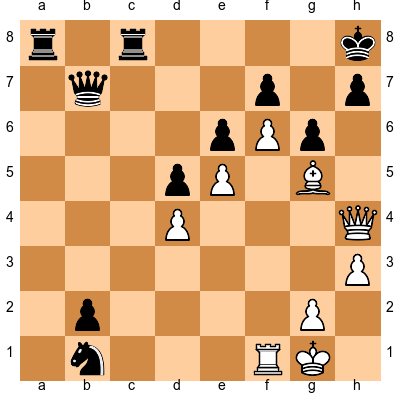
\includegraphics[width=8cm,height=8cm]{chess.png}};

\pic[shift={(0,0,0)}] at (0,0,0) 
    {Box={
        name=conv_block1,
        caption=\makebox[0pt]{\shortstack[c]{Conv2d\\BN\\Relu}},
        xlabel={{64, }},
        zlabel=8,
        fill=\ConvColor,
        height=35,
        width=2,
        depth=35
        }
    };

\pic[shift={ (0,0,0) }] at (conv_block1-east) 
    {Box={
        name=conv_block1_batchnorm,
        caption=,
        fill=\BatchNormColor,
        height=35,
        width=0.6666666666666666,
        depth=35
        }
    };

\pic[shift={ (0,0,0) }] at (conv_block1_batchnorm-east) 
    {Box={
        name=conv_block1_relu,
        caption=,
        fill=\ConvReluColor,
        opacity=0.5,
        height=35,
        width=0.5,
        depth=35
        }
    };

\pic[shift={(2,0,0)}] at (conv_block1_relu-east) 
    {Box={
        name=res_0_conv_1,
        caption=\makebox[0pt]{\shortstack[c]{Conv2d\\BN\\Relu}},
        xlabel={{64, }},
        zlabel=8,
        fill=\ConvColor,
        height=35,
        width=2,
        depth=35
        }
    };

\pic[shift={ (0,0,0) }] at (res_0_conv_1-east) 
    {Box={
        name=res_0_conv_1_batchnorm,
        caption=,
        fill=\BatchNormColor,
        height=35,
        width=0.6666666666666666,
        depth=35
        }
    };

\pic[shift={ (0,0,0) }] at (res_0_conv_1_batchnorm-east) 
    {Box={
        name=res_0_conv_1_relu,
        caption=,
        fill=\ConvReluColor,
        opacity=0.5,
        height=35,
        width=0.5,
        depth=35
        }
    };

\draw [connection]  (conv_block1_relu-east)    -- node {\midarrow} (res_0_conv_1-west);

\pic[shift={(1,0,0)}] at (res_0_conv_1-east) 
    {Box={
        name=res_0_conv_2,
        caption=\makebox[0pt]{\shortstack[c]{Conv2d\\BN}},
        xlabel={{64, }},
        zlabel=8,
        fill=\ConvColor,
        height=35,
        width=2,
        depth=35
        }
    };

\pic[shift={ (0,0,0) }] at (res_0_conv_2-east) 
    {Box={
        name=res_0_conv_2_batchnorm,
        caption= ,
        fill=\BatchNormColor,
        height=35,
        width=0.6666666666666666,
        depth=35
        }
    };

\draw [connection]  (res_0_conv_1-east)    -- node {\midarrow} (res_0_conv_2-west);

\pic[shift={ (1,0,0) }] at (res_0_conv_2-east) 
    {Box={
        name=res_0_se,
        caption=\makebox[0pt]{\shortstack[c]{SE}},
        xlabel={{64, }},
        ylabel=8,
        fill=\OpoolColor,
        height=35,
        width=2,
        depth=35
        }
	};

\draw [connection]  (res_0_conv_2-east)    -- node {\midarrow} (res_0_se-west);

\pic[shift={(1,0,0)}] at (res_0_se-east) 
    {Box={
        name=res_0_skip,
        caption=\makebox[0pt]{\shortstack[c]{Add\\Relu}},
        xlabel={{64, }},
        zlabel=8,
        fill=\ConvColor,
        height=35,
        width=2,
        depth=35
        }
    };

\pic[shift={ (0,0,0) }] at (res_0_skip-east) 
    {Ball={
        name=res_0_add,
        caption= ,
        fill=\SumColor,
        opacity=0.6,
        radius=2.5,
        logo=\(+\),
        }
    };

\pic[shift={ (0,0,0) }] at (res_0_skip-east) 
    {Box={
        name=res_0_add_relu,
        caption= ,
        fill=\ConvReluColor,
        opacity=0.5,
        height=35,
        width=0.5,
        depth=35
        }
    };

\draw [connection]  (res_0_se-east)    -- node {\midarrow} (res_0_skip-west);

\path (res_0_conv_1-south) -- (res_0_conv_1-north) coordinate[pos=1.25] (res_0_conv_1-top) ;
\path (res_0_skip-south)  -- (res_0_skip-north)  coordinate[pos=1.25] (res_0_skip-top) ;
\draw [copyconnection]  (res_0_conv_1-north)  
-- node {\copymidarrow}(res_0_conv_1-top)
-- node {\copymidarrow}(res_0_skip-top)
-- node {\copymidarrow} (res_0_skip-north);

\pic[shift={(2,0,0)}] at (res_0_skip-east) 
    {Box={
        name=res_1_conv_1,
        caption=\makebox[0pt]{\shortstack[c]{Conv2d\\BN\\Relu}},
        xlabel={{64, }},
        zlabel=8,
        fill=\ConvColor,
        height=35,
        width=2,
        depth=35
        }
    };

\pic[shift={ (0,0,0) }] at (res_1_conv_1-east) 
    {Box={
        name=res_1_conv_1_batchnorm,
        caption=,
        fill=\BatchNormColor,
        height=35,
        width=0.6666666666666666,
        depth=35
        }
    };

\pic[shift={ (0,0,0) }] at (res_1_conv_1_batchnorm-east) 
    {Box={
        name=res_1_conv_1_relu,
        caption=,
        fill=\ConvReluColor,
        opacity=0.5,
        height=35,
        width=0.5,
        depth=35
        }
    };

\draw [connection]  (res_0_skip-east)    -- node {\midarrow} (res_1_conv_1-west);

\pic[shift={(1,0,0)}] at (res_1_conv_1-east) 
    {Box={
        name=res_1_conv_2,
        caption=\makebox[0pt]{\shortstack[c]{Conv2d\\BN}},
        xlabel={{64, }},
        zlabel=8,
        fill=\ConvColor,
        height=35,
        width=2,
        depth=35
        }
    };

\pic[shift={ (0,0,0) }] at (res_1_conv_2-east) 
    {Box={
        name=res_1_conv_2_batchnorm,
        caption= ,
        fill=\BatchNormColor,
        height=35,
        width=0.6666666666666666,
        depth=35
        }
    };

\draw [connection]  (res_1_conv_1-east)    -- node {\midarrow} (res_1_conv_2-west);

\pic[shift={ (1,0,0) }] at (res_1_conv_2-east) 
    {Box={
        name=res_1_se,
        caption=\makebox[0pt]{\shortstack[c]{SE}},
        xlabel={{64, }},
        ylabel=8,
        fill=\OpoolColor,
        height=35,
        width=2,
        depth=35
        }
	};

\draw [connection]  (res_1_conv_2-east)    -- node {\midarrow} (res_1_se-west);

\pic[shift={(1,0,0)}] at (res_1_se-east) 
    {Box={
        name=res_1_skip,
        caption=\makebox[0pt]{\shortstack[c]{Add\\Relu}},
        xlabel={{64, }},
        zlabel=8,
        fill=\ConvColor,
        height=35,
        width=2,
        depth=35
        }
    };

\pic[shift={ (0,0,0) }] at (res_1_skip-east) 
    {Ball={
        name=res_1_add,
        caption= ,
        fill=\SumColor,
        opacity=0.6,
        radius=2.5,
        logo=\(+\),
        }
    };

\pic[shift={ (0,0,0) }] at (res_1_skip-east) 
    {Box={
        name=res_1_add_relu,
        caption= ,
        fill=\ConvReluColor,
        opacity=0.5,
        height=35,
        width=0.5,
        depth=35
        }
    };

\draw [connection]  (res_1_se-east)    -- node {\midarrow} (res_1_skip-west);

\path (res_1_conv_1-south) -- (res_1_conv_1-north) coordinate[pos=1.25] (res_1_conv_1-top) ;
\path (res_1_skip-south)  -- (res_1_skip-north)  coordinate[pos=1.25] (res_1_skip-top) ;
\draw [copyconnection]  (res_1_conv_1-north)  
-- node {\copymidarrow}(res_1_conv_1-top)
-- node {\copymidarrow}(res_1_skip-top)
-- node {\copymidarrow} (res_1_skip-north);

\pic[shift={(2,0,0)}] at (res_1_skip-east) 
    {Box={
        name=res_2_conv_1,
        caption=\makebox[0pt]{\shortstack[c]{Conv2d\\BN\\Relu}},
        xlabel={{64, }},
        zlabel=8,
        fill=\ConvColor,
        height=35,
        width=2,
        depth=35
        }
    };

\pic[shift={ (0,0,0) }] at (res_2_conv_1-east) 
    {Box={
        name=res_2_conv_1_batchnorm,
        caption=,
        fill=\BatchNormColor,
        height=35,
        width=0.6666666666666666,
        depth=35
        }
    };

\pic[shift={ (0,0,0) }] at (res_2_conv_1_batchnorm-east) 
    {Box={
        name=res_2_conv_1_relu,
        caption=,
        fill=\ConvReluColor,
        opacity=0.5,
        height=35,
        width=0.5,
        depth=35
        }
    };

\draw [connection]  (res_1_skip-east)    -- node {\midarrow} (res_2_conv_1-west);

\pic[shift={(1,0,0)}] at (res_2_conv_1-east) 
    {Box={
        name=res_2_conv_2,
        caption=\makebox[0pt]{\shortstack[c]{Conv2d\\BN}},
        xlabel={{64, }},
        zlabel=8,
        fill=\ConvColor,
        height=35,
        width=2,
        depth=35
        }
    };

\pic[shift={ (0,0,0) }] at (res_2_conv_2-east) 
    {Box={
        name=res_2_conv_2_batchnorm,
        caption= ,
        fill=\BatchNormColor,
        height=35,
        width=0.6666666666666666,
        depth=35
        }
    };

\draw [connection]  (res_2_conv_1-east)    -- node {\midarrow} (res_2_conv_2-west);

\pic[shift={ (1,0,0) }] at (res_2_conv_2-east) 
    {Box={
        name=res_2_se,
        caption=\makebox[0pt]{\shortstack[c]{SE}},
        xlabel={{64, }},
        ylabel=8,
        fill=\OpoolColor,
        height=35,
        width=2,
        depth=35
        }
	};

\draw [connection]  (res_2_conv_2-east)    -- node {\midarrow} (res_2_se-west);

\pic[shift={(1,0,0)}] at (res_2_se-east) 
    {Box={
        name=res_2_skip,
        caption=\makebox[0pt]{\shortstack[c]{Add\\Relu}},
        xlabel={{64, }},
        zlabel=8,
        fill=\ConvColor,
        height=35,
        width=2,
        depth=35
        }
    };

\pic[shift={ (0,0,0) }] at (res_2_skip-east) 
    {Ball={
        name=res_2_add,
        caption= ,
        fill=\SumColor,
        opacity=0.6,
        radius=2.5,
        logo=\(+\),
        }
    };

\pic[shift={ (0,0,0) }] at (res_2_skip-east) 
    {Box={
        name=res_2_add_relu,
        caption= ,
        fill=\ConvReluColor,
        opacity=0.5,
        height=35,
        width=0.5,
        depth=35
        }
    };

\draw [connection]  (res_2_se-east)    -- node {\midarrow} (res_2_skip-west);

\path (res_2_conv_1-south) -- (res_2_conv_1-north) coordinate[pos=1.25] (res_2_conv_1-top) ;
\path (res_2_skip-south)  -- (res_2_skip-north)  coordinate[pos=1.25] (res_2_skip-top) ;
\draw [copyconnection]  (res_2_conv_1-north)  
-- node {\copymidarrow}(res_2_conv_1-top)
-- node {\copymidarrow}(res_2_skip-top)
-- node {\copymidarrow} (res_2_skip-north);

\pic[shift={(2,0,0)}] at (res_2_skip-east) 
    {Box={
        name=res_3_conv_1,
        caption=\makebox[0pt]{\shortstack[c]{Conv2d\\BN\\Relu}},
        xlabel={{64, }},
        zlabel=8,
        fill=\ConvColor,
        height=35,
        width=2,
        depth=35
        }
    };

\pic[shift={ (0,0,0) }] at (res_3_conv_1-east) 
    {Box={
        name=res_3_conv_1_batchnorm,
        caption=,
        fill=\BatchNormColor,
        height=35,
        width=0.6666666666666666,
        depth=35
        }
    };

\pic[shift={ (0,0,0) }] at (res_3_conv_1_batchnorm-east) 
    {Box={
        name=res_3_conv_1_relu,
        caption=,
        fill=\ConvReluColor,
        opacity=0.5,
        height=35,
        width=0.5,
        depth=35
        }
    };

\draw [connection]  (res_2_skip-east)    -- node {\midarrow} (res_3_conv_1-west);

\pic[shift={(1,0,0)}] at (res_3_conv_1-east) 
    {Box={
        name=res_3_conv_2,
        caption=\makebox[0pt]{\shortstack[c]{Conv2d\\BN}},
        xlabel={{64, }},
        zlabel=8,
        fill=\ConvColor,
        height=35,
        width=2,
        depth=35
        }
    };

\pic[shift={ (0,0,0) }] at (res_3_conv_2-east) 
    {Box={
        name=res_3_conv_2_batchnorm,
        caption= ,
        fill=\BatchNormColor,
        height=35,
        width=0.6666666666666666,
        depth=35
        }
    };

\draw [connection]  (res_3_conv_1-east)    -- node {\midarrow} (res_3_conv_2-west);

\pic[shift={ (1,0,0) }] at (res_3_conv_2-east) 
    {Box={
        name=res_3_se,
        caption=\makebox[0pt]{\shortstack[c]{SE}},
        xlabel={{64, }},
        ylabel=8,
        fill=\OpoolColor,
        height=35,
        width=2,
        depth=35
        }
	};

\draw [connection]  (res_3_conv_2-east)    -- node {\midarrow} (res_3_se-west);

\pic[shift={(1,0,0)}] at (res_3_se-east) 
    {Box={
        name=res_3_skip,
        caption=\makebox[0pt]{\shortstack[c]{Add\\Relu}},
        xlabel={{64, }},
        zlabel=8,
        fill=\ConvColor,
        height=35,
        width=2,
        depth=35
        }
    };

\pic[shift={ (0,0,0) }] at (res_3_skip-east) 
    {Ball={
        name=res_3_add,
        caption= ,
        fill=\SumColor,
        opacity=0.6,
        radius=2.5,
        logo=\(+\),
        }
    };

\pic[shift={ (0,0,0) }] at (res_3_skip-east) 
    {Box={
        name=res_3_add_relu,
        caption= ,
        fill=\ConvReluColor,
        opacity=0.5,
        height=35,
        width=0.5,
        depth=35
        }
    };

\draw [connection]  (res_3_se-east)    -- node {\midarrow} (res_3_skip-west);

\path (res_3_conv_1-south) -- (res_3_conv_1-north) coordinate[pos=1.25] (res_3_conv_1-top) ;
\path (res_3_skip-south)  -- (res_3_skip-north)  coordinate[pos=1.25] (res_3_skip-top) ;
\draw [copyconnection]  (res_3_conv_1-north)  
-- node {\copymidarrow}(res_3_conv_1-top)
-- node {\copymidarrow}(res_3_skip-top)
-- node {\copymidarrow} (res_3_skip-north);

\pic[shift={(2,0,0)}] at (res_3_skip-east) 
    {Box={
        name=res_4_conv_1,
        caption=\makebox[0pt]{\shortstack[c]{Conv2d\\BN\\Relu}},
        xlabel={{64, }},
        zlabel=8,
        fill=\ConvColor,
        height=35,
        width=2,
        depth=35
        }
    };

\pic[shift={ (0,0,0) }] at (res_4_conv_1-east) 
    {Box={
        name=res_4_conv_1_batchnorm,
        caption=,
        fill=\BatchNormColor,
        height=35,
        width=0.6666666666666666,
        depth=35
        }
    };

\pic[shift={ (0,0,0) }] at (res_4_conv_1_batchnorm-east) 
    {Box={
        name=res_4_conv_1_relu,
        caption=,
        fill=\ConvReluColor,
        opacity=0.5,
        height=35,
        width=0.5,
        depth=35
        }
    };

\draw [connection]  (res_3_skip-east)    -- node {\midarrow} (res_4_conv_1-west);

\pic[shift={(1,0,0)}] at (res_4_conv_1-east) 
    {Box={
        name=res_4_conv_2,
        caption=\makebox[0pt]{\shortstack[c]{Conv2d\\BN}},
        xlabel={{64, }},
        zlabel=8,
        fill=\ConvColor,
        height=35,
        width=2,
        depth=35
        }
    };

\pic[shift={ (0,0,0) }] at (res_4_conv_2-east) 
    {Box={
        name=res_4_conv_2_batchnorm,
        caption= ,
        fill=\BatchNormColor,
        height=35,
        width=0.6666666666666666,
        depth=35
        }
    };

\draw [connection]  (res_4_conv_1-east)    -- node {\midarrow} (res_4_conv_2-west);

\pic[shift={ (1,0,0) }] at (res_4_conv_2-east) 
    {Box={
        name=res_4_se,
        caption=\makebox[0pt]{\shortstack[c]{SE}},
        xlabel={{64, }},
        ylabel=8,
        fill=\OpoolColor,
        height=35,
        width=2,
        depth=35
        }
	};

\draw [connection]  (res_4_conv_2-east)    -- node {\midarrow} (res_4_se-west);

\pic[shift={(1,0,0)}] at (res_4_se-east) 
    {Box={
        name=res_4_skip,
        caption=\makebox[0pt]{\shortstack[c]{Add\\Relu}},
        xlabel={{64, }},
        zlabel=8,
        fill=\ConvColor,
        height=35,
        width=2,
        depth=35
        }
    };

\pic[shift={ (0,0,0) }] at (res_4_skip-east) 
    {Ball={
        name=res_4_add,
        caption= ,
        fill=\SumColor,
        opacity=0.6,
        radius=2.5,
        logo=\(+\),
        }
    };

\pic[shift={ (0,0,0) }] at (res_4_skip-east) 
    {Box={
        name=res_4_add_relu,
        caption= ,
        fill=\ConvReluColor,
        opacity=0.5,
        height=35,
        width=0.5,
        depth=35
        }
    };

\draw [connection]  (res_4_se-east)    -- node {\midarrow} (res_4_skip-west);

\path (res_4_conv_1-south) -- (res_4_conv_1-north) coordinate[pos=1.25] (res_4_conv_1-top) ;
\path (res_4_skip-south)  -- (res_4_skip-north)  coordinate[pos=1.25] (res_4_skip-top) ;
\draw [copyconnection]  (res_4_conv_1-north)  
-- node {\copymidarrow}(res_4_conv_1-top)
-- node {\copymidarrow}(res_4_skip-top)
-- node {\copymidarrow} (res_4_skip-north);

\pic[shift={(2,0,0)}] at (res_4_skip-east) 
    {Box={
        name=res_5_conv_1,
        caption=\makebox[0pt]{\shortstack[c]{Conv2d\\BN\\Relu}},
        xlabel={{64, }},
        zlabel=8,
        fill=\ConvColor,
        height=35,
        width=2,
        depth=35
        }
    };

\pic[shift={ (0,0,0) }] at (res_5_conv_1-east) 
    {Box={
        name=res_5_conv_1_batchnorm,
        caption=,
        fill=\BatchNormColor,
        height=35,
        width=0.6666666666666666,
        depth=35
        }
    };

\pic[shift={ (0,0,0) }] at (res_5_conv_1_batchnorm-east) 
    {Box={
        name=res_5_conv_1_relu,
        caption=,
        fill=\ConvReluColor,
        opacity=0.5,
        height=35,
        width=0.5,
        depth=35
        }
    };

\draw [connection]  (res_4_skip-east)    -- node {\midarrow} (res_5_conv_1-west);

\pic[shift={(1,0,0)}] at (res_5_conv_1-east) 
    {Box={
        name=res_5_conv_2,
        caption=\makebox[0pt]{\shortstack[c]{Conv2d\\BN}},
        xlabel={{64, }},
        zlabel=8,
        fill=\ConvColor,
        height=35,
        width=2,
        depth=35
        }
    };

\pic[shift={ (0,0,0) }] at (res_5_conv_2-east) 
    {Box={
        name=res_5_conv_2_batchnorm,
        caption= ,
        fill=\BatchNormColor,
        height=35,
        width=0.6666666666666666,
        depth=35
        }
    };

\draw [connection]  (res_5_conv_1-east)    -- node {\midarrow} (res_5_conv_2-west);

\pic[shift={ (1,0,0) }] at (res_5_conv_2-east) 
    {Box={
        name=res_5_se,
        caption=\makebox[0pt]{\shortstack[c]{SE}},
        xlabel={{64, }},
        ylabel=8,
        fill=\OpoolColor,
        height=35,
        width=2,
        depth=35
        }
	};

\draw [connection]  (res_5_conv_2-east)    -- node {\midarrow} (res_5_se-west);

\pic[shift={(1,0,0)}] at (res_5_se-east) 
    {Box={
        name=res_5_skip,
        caption=\makebox[0pt]{\shortstack[c]{Add\\Relu}},
        xlabel={{64, }},
        zlabel=8,
        fill=\ConvColor,
        height=35,
        width=2,
        depth=35
        }
    };

\pic[shift={ (0,0,0) }] at (res_5_skip-east) 
    {Ball={
        name=res_5_add,
        caption= ,
        fill=\SumColor,
        opacity=0.6,
        radius=2.5,
        logo=\(+\),
        }
    };

\pic[shift={ (0,0,0) }] at (res_5_skip-east) 
    {Box={
        name=res_5_add_relu,
        caption= ,
        fill=\ConvReluColor,
        opacity=0.5,
        height=35,
        width=0.5,
        depth=35
        }
    };

\draw [connection]  (res_5_se-east)    -- node {\midarrow} (res_5_skip-west);

\path (res_5_conv_1-south) -- (res_5_conv_1-north) coordinate[pos=1.25] (res_5_conv_1-top) ;
\path (res_5_skip-south)  -- (res_5_skip-north)  coordinate[pos=1.25] (res_5_skip-top) ;
\draw [copyconnection]  (res_5_conv_1-north)  
-- node {\copymidarrow}(res_5_conv_1-top)
-- node {\copymidarrow}(res_5_skip-top)
-- node {\copymidarrow} (res_5_skip-north);

\pic[shift={(4.5,4.5,0)}] at (res_5_add_relu-east) 
    {Box={
        name=policy_head_conv_1,
        caption=\makebox[0pt]{\shortstack[c]{Conv2d\\BN\\Relu}},
        xlabel={{64, }},
        zlabel=8,
        fill=\ConvColor,
        height=35,
        width=2,
        depth=35
        }
    };

\pic[shift={ (0,0,0) }] at (policy_head_conv_1-east) 
    {Box={
        name=policy_head_conv_1_batchnorm,
        caption=,
        fill=\BatchNormColor,
        height=35,
        width=0.6666666666666666,
        depth=35
        }
    };

\pic[shift={ (0,0,0) }] at (policy_head_conv_1_batchnorm-east) 
    {Box={
        name=policy_head_conv_1_relu,
        caption=,
        fill=\ConvReluColor,
        opacity=0.5,
        height=35,
        width=0.5,
        depth=35
        }
    };

    \draw [connection] (res_5_add_relu-north) -- node {\midarrow} (res_5_add_relu-north|-policy_head_conv_1-west) -- node {\midarrow} (policy_head_conv_1-west) ;

\pic[shift={(2.4,0,0)}] at (policy_head_conv_1-east) 
    {Box={
        name=policy_head_conv_2,
        caption=\makebox[0pt]{\shortstack[c]{Conv2d}},
        xlabel={{80, }},
        zlabel=8,
        fill=\ConvColor,
        height=35,
        width=4,
        depth=35
        }
    };

\draw [connection]  (policy_head_conv_1-east)    -- node {\midarrow} (policy_head_conv_2-west);

\pic[shift={ (2.3,0,0) }] at (policy_head_conv_2-east) 
    {RightBandedBox={
        name=policy_head_policy_map,
        caption=\makebox[0pt]{\shortstack[c]{ \\ \\ \\ Reshape\\PolicyMap\\Softmax}},
        xlabel={{1858, }},
        zlabel=1,
        fill=\FcColor,
        bandfill=\SoftmaxColor,
        height=4.5,
        width=14,
        depth=4.5
        }
	};

\draw [densely dashed] 
(policy_head_policy_map-west)++(0, 1.5*.2 * 1.5, 1.5*.2 * 1.5) coordinate(a) -- (policy_head_conv_2-nearnortheast)
(policy_head_policy_map-west)++(0,-1.5*.2 * 1.5, 1.5*.2 * 1.5) coordinate(b) -- (policy_head_conv_2-nearsoutheast)
(policy_head_policy_map-west)++(0,-1.5*.2 * 1.5,-1.5*.2 * 1.5) coordinate(c) -- (policy_head_conv_2-farsoutheast)
(policy_head_policy_map-west)++(0, 1.5*.2 * 1.5,-1.5*.2 * 1.5) coordinate(d) -- (policy_head_conv_2-farnortheast)

(a)--(b)--(c)--(d)
;

\pic[shift={ (2.3,0,0) }] at (policy_head_policy_map-east) 
    {Box={
        name=policy_head_output,
        caption=\makebox[0pt]{\shortstack[c]{Policy Output\\Qh6}},
        xlabel={{1, }},
        zlabel=1,
        fill=\FcColor,
        height=4.5,
        width=4.5,
        depth=4.5
        }
	};

\draw [densely dashed]  (policy_head_policy_map-east)    -- node {\midarrow} (policy_head_output-west);

\pic[shift={ (2,-4.5,0) }] at (res_5_add_relu-east) 
    {Box={
        name=invisible,
        caption= ,
        fill=\ConvReluColor,
        opacity=0,
        height=0,
        width=0,
        depth=0
        }
    };

    \draw [brokenconnection] (res_5_add_relu-south) -- node {\brokenmidarrow} (res_5_add_relu-south|-invisible-west) -- node {\brokenmidarrow}  (invisible-west) ;

\draw (invisible-east) node[cross] {};

\pic[shift={(2.5,0,0)}] at (invisible-east) 
    {Box={
        name=value_head_conv_1,
        caption=\makebox[0pt]{\shortstack[c]{Conv2d\\BN\\Relu}},
        xlabel={{32, }},
        zlabel=8,
        fill=\ConvColor,
        height=35,
        width=1.5,
        depth=35
        }
    };

\pic[shift={ (0,0,0) }] at (value_head_conv_1-east) 
    {Box={
        name=value_head_conv_1_batchnorm,
        caption=,
        fill=\BatchNormColor,
        height=35,
        width=0.5,
        depth=35
        }
    };

\pic[shift={ (0,0,0) }] at (value_head_conv_1_batchnorm-east) 
    {Box={
        name=value_head_conv_1_relu,
        caption=,
        fill=\ConvReluColor,
        opacity=0.5,
        height=35,
        width=0.375,
        depth=35
        }
    };

\draw [brokenconnection]  (invisible-east)    -- node {\brokenmidarrow} (value_head_conv_1-west);

\pic[shift={ (2.5,0,0) }] at (value_head_conv_1-east) 
    {Box={
        name=value_head_dense1,
        caption=\makebox[0pt]{\shortstack[c]{Flatten\\Fully Connected}},
        xlabel={{128, }},
        zlabel=1,
        fill=\FcColor,
        height=4.5,
        width=8.25,
        depth=4.5
        }
	};

\draw [densely dashed] 
(value_head_dense1-west)++(0, 1.5*.2 * 1.5, 1.5*.2 * 1.5) coordinate(a) -- (value_head_conv_1-nearnortheast)
(value_head_dense1-west)++(0,-1.5*.2 * 1.5, 1.5*.2 * 1.5) coordinate(b) -- (value_head_conv_1-nearsoutheast)
(value_head_dense1-west)++(0,-1.5*.2 * 1.5,-1.5*.2 * 1.5) coordinate(c) -- (value_head_conv_1-farsoutheast)
(value_head_dense1-west)++(0, 1.5*.2 * 1.5,-1.5*.2 * 1.5) coordinate(d) -- (value_head_conv_1-farnortheast)

(a)--(b)--(c)--(d)
;

\pic[shift={ (2.5,0,0) }] at (value_head_dense1-east) 
    {RightBandedBox={
        name=value_head_dense2,
        caption=\makebox[0pt]{\shortstack[c]{Fully Connected\\Softmax}},
        xlabel={{3, }},
        zlabel=1,
        fill=\FcColor,
        bandfill=\SoftmaxColor,
        height=4.5,
        width=6.75,
        depth=4.5
        }
	};

\draw [connection]  (value_head_dense1-east)    -- node {\midarrow} (value_head_dense2-west);

\pic[shift={ (2.5,0,0) }] at (value_head_dense2-east) 
    {Box={
        name=value_head_output,
        caption=\makebox[0pt]{\shortstack[c]{Value Output\\80\% to win}},
        xlabel={{1, }},
        zlabel=1,
        fill=\FcColor,
        height=4.5,
        width=4.5,
        depth=4.5
        }
	};

\draw [densely dashed]  (value_head_dense2-east)    -- node {\midarrow} (value_head_output-west);

\end{tikzpicture}
\end{document}
